%% chapter was hard to write b/c
% - survery of surveys 
% - conflicting information
% - little indication of what method to use for what kind of data
\chapter[adts]{Anomaly Detection in Time Series}

\section[adintro]{Introduction}

The goal of this chapter is to show that the solution to the general problem of anomaly detection in time series is difficult. A typical general framework for anomaly detection in time series is explained with two advanced solutions as examples and their issues. The proposed solution, explained later, fits into the framework providing a basis for comparison.

Describing the variety of solutions puts this difficulty in context. Few publications survery the problem of anomaly detection for time series in particular \cite{Cheboli2010} \cite{Gupta2013}.

Solutions have been fragmented across a variety of application domains such as communication networks \cite{Jiang2006, Szymanski2004, Ye2000, Portnoy2001, Zhen2006, Warrender1999, Angiulli2007, Lane1999, Lane1997, Hofmeyr1998, Sequeira2002}, economics \cite{gupta2012community, Otey2006, Zhu2003}, environmental science \cite{Hill2010, Hill2010a, Angiulli2007, Birant2006, Cheng2006, Yuxiang2005, Wu2010, Drosdowsky1993, Lasaponara2006, Lu2004}, industrial process \cite{Basu2007, Nairac1999, Dasgupta1996, Bu2007}, biology \cite{Keogh2005, Wei2006}, astronomy \cite{Keogh2005, Yankov2008}, and transportation \cite{Li2009,Ge2010}. The fragmentation of application domains led to a variety of problem formulations \cite{Gupta2013}. Furthermore, there is no good understanding of how the solutions in different application domains compare to each other \cite{Cheboli2010}. Therefore, it is difficult to generalize the performance of a solution formulated in one application domain to its performance in another although they might have common elements at a higher level.

Furthmore, adding to the difficulty of comparing solutions, the mechanics of anomaly detection have come from two disciplines: statistics and computer science. Solutions from statistics focus on mathematical rigor while solutions from computer science consider computational issues \cite{Gupta2013}.

\cite{Gupta2013} offers a survey of of anomaly detection problems in a variety of settings such as streaming data, distributed data, and databases. To focus the solution presented here, the problem will be stated as follows: given a finite time series $X$
 \[ X=\{X_1,X_2,X_t,\ldots,X_T\}\]
\[  X \in \mathbb{R}^n \]
where $T$ is the length of the regularly spaced sequence and $n$ is the number of variables $X$ can have, find points in which can be considered anomalous. This statement makes sense only when anomlous points are a small part of the data. Furthermore, anomalies may not even be present.

So elements of any solution to this problem must answer the following questions:

\begin{enumerate}
\item
What is normal (as an anomaly is defined as what is \textit{not} normal)?
\item
What measure is used to indicate how anomalous point(s) are?
\item
How is the measure tested to decide if it is anomalous?
\end{enumerate}



\section[adtypes]{Anomaly Types}

The presense of different anomaly types can be a challenge for anomaly detection techniques. What follow are qualitative descriptions of anomalies classified in a way most relevent to this thesis. However, a taxonomy of anomalies will never encompass all anomalies as well as defining anomalies as points that are not normal.

\subsection[ptanom]{Point Anomalies}

Point anomalies are single points of interest.

\textbf{Simple:} Simple point anomalies are just defined by their value. They are trivial to describe and detect. They are not of much interest in themselves but are mentioned because anomlaies in more complicated time series can be `converted' to resemble this simple type.

\begin{figure}[H]
  \centering
  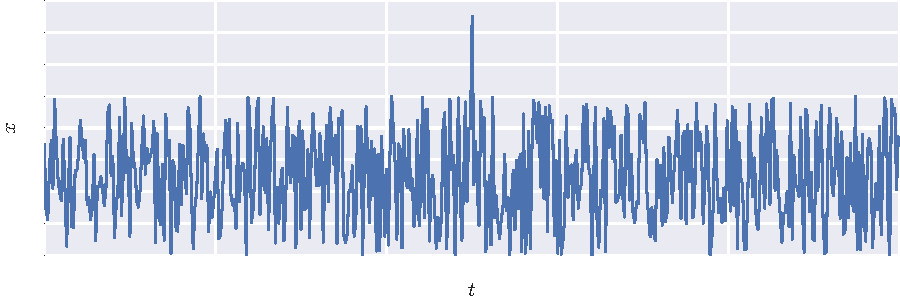
\includegraphics{figs/trivial.pdf}
  \caption{Simple Point Anomaly}
\end{figure}


\textbf{Context:} Some anomalies are defined within a context. In Figure \ref{fig:contextanom}, the anomalous point's value is within the range of the overall time series. But if the cyclic nature of the series were removed, the anomaly is readily detected (`converted' to a simple point anomaly).

\begin{figure}[H]
  \centering
  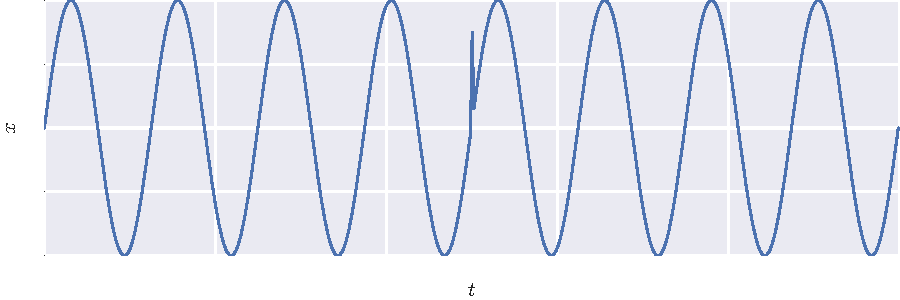
\includegraphics{figs/context.pdf}
  \caption{Anomaly in a Periodic Context}
  \label{fig:contextanom}
\end{figure}


\subsection{Discord}

Anomalies over subsequences are called discords \cite{Cheboli2010}. In Figure \ref{fig:perdiscordanom}, about two cycles in a periodic time series are unlike the other cycles. The repeated units do not have to be periodic as in Figure \ref{fig:aperdiscordanom}. 

\begin{figure}[H]
  \centering
  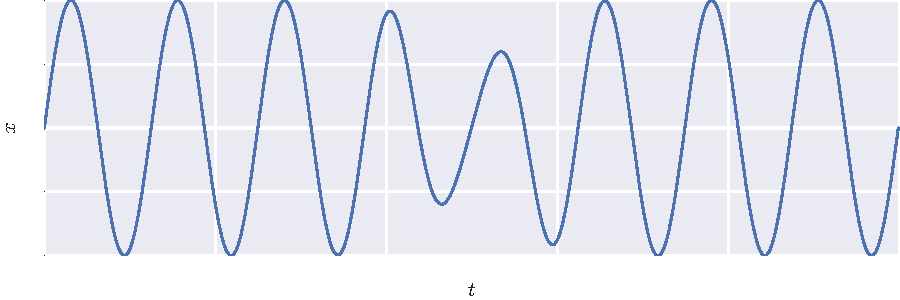
\includegraphics{figs/discord_per.pdf}
  \caption{Discord Anomaly in a Periodic Time Series}
  \label{fig:perdiscordanom}
\end{figure}

\begin{figure}[H]
  \centering
  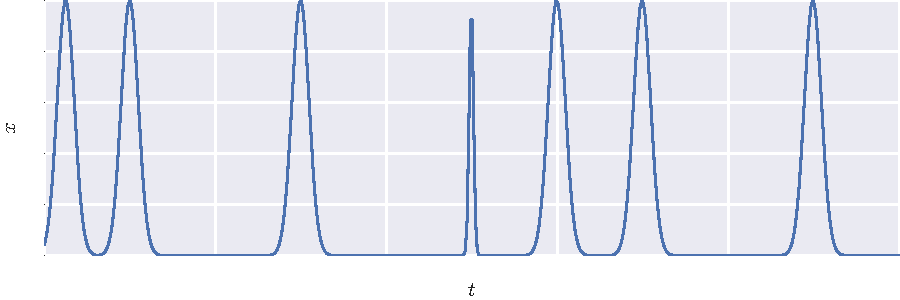
\includegraphics{figs/discord_aper.pdf}
  \caption{Discord Anomaly in an Aperiodic Time Series}
  \label{fig:aperdiscordanom}
\end{figure}

\subsection{Multivariate}

Multivariate \footnote{In this text, dimensionality of the time series will refer to the length of the time series as opposed to the number of its variables. Time series anomaly detection literature is inconsistent in the terminology used to refer to these two attributes.} time series add another element of complication for detecting anomalies in them and are not a focus of the thesis. \cite{Cheboli2010} classifies multivariate time series according to a combination of periodicity and synchronicity: Variables in a time series can be synchronous and periodic, syncronous and aperiodic, asynchronous and periodic, asyncronous and aperiodic. Therefore, any deviation from these properties are anomalies.




\section[adproc]{Detection Technique}


In this section, a procedure to find anomalies in time series will be outlined to help answer the questions posed in the introduction of this chapter. The focus will be on issues related to time series as opposed to the general anomaly detection problem. However, there will be a focus on the issues related to solving the general problem of finding anomalies in (an arbitrary) time series as opposed to finding anomalies in a particular application domain. Also, computational issues will not be emphasized.

By examining many detection techniques, a general procedure (Section 2.7 in \cite{Cheboli2010}) can be gleaned:

\begin{enumerate}
\item Compute an anomaly score for an observation (a point or a subsequence in a time series). The anomaly score is a deviation from some `normal' value such as a model or similarity to other observations.
\item Aggregate the anomaly scores for many observations.
\item Use the anomaly scores to determine whether an observation can be considered anomalous. For example, an observation could be considered anomalous if its anomaly score exceeds three standard deviations of other anomaly scores.
\end{enumerate}

The procedure is rather straightforward. But, the process of finding what is normal is not. This section is devoted to explaining why finding anomalies in time series is particularly challenging. Addressing the stated problem, given an (single) arbitrary time series, the process of finding normal behaviour involves the following steps:
\begin{enumerate}
\item Extract Samples
\item Transform Samples
\item Apply Detection Technique
\end{enumerate}

\subsection{Sample Extraction}

Many instances of data are needed to inform what is normal. So, subsequences need to be extracted from a (long) sequence.

Samples can be extracted from a sliding a window over the time series. More precisely, beginning at step $t=0$, sliding a window of width $w$ over a time series $X$ of length $T$ one step at a time produces $p=T-w+1$ windows, $\mathcal{X}=\{W_1,W_2,\ldots,W_p\}$\footnote{In literature, this form corresponds to a time series database \cite{Gupta2013}}.

Now, $\mathcal{X}$ contains all possible subsequences of $X$ of length $w$ and the value $p$ is typically not much less than $T$. Having many subsequences helps to localize the anomaly; so the window capturing the anomaly will have a higher anomaly score than adjacent windows.

But sometimes it is not desirable for computational reasons to process all subsequences. $p$ can be reduced by introducing a `hop', $h$, that skips $h$ steps when advancing the window from the previous one ($h=1$ gives all possible subsequences). 

However, by introduing a large enough hop, anomalies could be missed. Consider the sequence \emph{abccabcabc}. The second \emph{c} is an anomaly. Now inspect the windows generated by various values of $h$ in Table \ref{tbl:hop}. The anomalous \emph{c} is captured in a window when $h$ is 1 or 2 but not when $h$ is 3 or 4. As a general rule, when $h=1$, an anomaly would never be missed. But when $h>1$, there is a chance that anomalies would be missed.

\begin{table}[h]
  \centering
  \begin{tabular}{|c|c|}
    \hline
    hop ($h$) & Windows \\
    \hline
    \hline
    1 & \emph{abc},
        \emph{bcc}, 
        \emph{cca}, 
        \emph{cab},
        \emph{abc}, 
        \emph{bca},
        \emph{cab},
        \emph{abc} \\
    \hline
    2 & \emph{abc},
        \emph{cca},
        \emph{abc},
        \emph{cab} \\
    \hline
    3 & \emph{abc}, 
        \emph{cab},
        \emph{cab} \\
    \hline
    4 & \emph{abc}, 
        \emph{abc} \\
    \hline
  \end{tabular}
  \caption{Windows of width 3 for various hop sizes. From \cite{Cheboli2010}}
  \label{tbl:hop}
\end{table}

Another issue that needs to be considered when working with windows is that the window size must be large enough to capture an anomaly. Consider the sequence \emph{aaabbbccccaabbbcccaaabbbccc} where the fourth \emph{c} is anomalous. The window width must be at least 4 to capture the fourth \emph{c}. 

Now given $\mathcal{X}$ for some $w$, the problem may be posed as a multivariate anomaly detection problem. In this setting, assuming that $X$ is univariate, samples of $\mathcal{X}$ correspond to $w$ variables. However, doing so largely ignores the temporal nature of $X$. These issues will be discussed within the forthcoming parts of this chapter.

Finally, subsequent steps taken in the anomaly detection process may put restrictions on $h$ and $w$. For example, if the window size is too large, there may not be enough samples properly apply an anomlay detection technique.

\subsection{Transformation}

Anomalies can be more easily detected if the time series are analyzed in a different representation. Usually these representations are of lower fidelity but capture the essential characterists of the time series in certain cases. As a general example, a real-valued time series could be or should be discretized into a finite set of symbols or numbers to make use of techniques from text processing of bioinformatics. Or, it could be transformed into a different domain such as the frequency domain to make use of techniques from signal processing. As an added benefit, the tranformed time series need less computation given their reduced representation.

More specifically, the Symbolic Aggregate approXimation (SAX) \cite{Lin2007} is an example of time series discretization used to find anomalies in  \cite{Keogh2005}. While the Haar transform represents a transformation to the frequency domain \cite{Bu2007,fu2006finding} for the same purpose.

However, as a transformation only captures the essential characteristics of a time series, more subtle anomalies could be lost in the transformation process. For example, the anomaly in \ref{fig:contextanom} would be difficult to encode in terms of frequency. The anomaly is localized in time while oscillations (representing frequencies) are not. 

Another issue to consider is the similarity of the arrangment of time series `points' (like elements of $\mathcal{X}$) in the transformed space to that of the original space. Some anomaly detection techniques rely a certain distribution of points in a space. Suppose an anomaly detection technique works in $\mathbb{R}^w$ by identifying points that are far away from some normal cluster of points. This arrangement should also be present in the transformed space. Anomaly detection techniques of this type are introduced in the next section. %todo ref next'

However, a recent empirical study \cite{Wang2013} suggests that, in general, there is little to differentiate between numerous time series representations. Only spectral transformations applied to periodic series showed some advantage but only in certain cases.

\subsection[adtechnique]{Detection Technique}

Discussion of detection techniques are discussed as a separate chapter.

\chapter[adtechnique]{Detection Technique}

The application of anomaly detection in a wide variety of application domains have led to the development of numerous detection techniques. Each of these applications defines anomalies in a different way;  some  may only be interested in single anomalous points while others are more concerned about anomalous subsquences. Furthermore, techniques are developed drawing on theory from statistics, machine learning, data mining, information theory, and spectral theory.

A highest-level categorization of these techniques could be as follows. The categories are not exhaustive but capture a wide variety of techniques discussed in literature.

\begin{description}

\item[Segmentation] In a segmentation-based techniques, the time series is first split into homogeneous segments. Then a finite-state automation is trained to learn transition probabilities between segments. So, a segmented anomalous time series should not have high transition probability \cite{Salvador2005,mahoney2005trajectory,Chan2005}.

\item[Information Theory] Information-theoretic techniques quantify a notion of information content such as entropy. So, a point is considered an anomaly if its removal reduces the information content significantly \cite{Muthukrishnan2004,jagadish1999mining}. That is, anomalous points increase disorder, or require more information to be represented in the sequence.

\item[Proximity] Techniques based on proximity map time series onto a space. It is expected that anomalous time series are `different' because they are far from normal ones.

\item[Model] The difference between the (actual) values of a time series and its predicted values from a model indicate how anomoulous they are.
 
\end{description}


Given the variety of techniques applied in different application domains, it is not always possible to use a solution developed for one problem and apply it to another. Finding a general anomaly detection technique is difficult. To the author's knowledge, only one study \cite{Cheboli2010} attempted to compare anomaly detection techniques over a wide variety of data. The study showed, as expected, varying performance of the techniques. Some explanations were given for the varying performance due to a combination of time series characteristics and algorithm settings. These explanations do not help to objectively determine \emph{a priori} what technique to use and how to adjust any parameters it might use.

It would be difficult to use information theoretic techniques because finding an information theoretic measure sensitive enough to detect a few anomalies is challenging \cite{Chandola2009}. Segmentation-based techniques require that a time series to be made of homogenous segments. These conditions are deemed too restrictive to be able to solve the general problem. In addition, both are not well-studied. So, they are not further explored here.

This leaves model-based techniques and proximity-based techniqes as potential solution categories. Both are widely studied. Furthermore, it is possible to make a theoretical comparison between model-based techniques and proximity-based techniques if they are evaluated as, respectively, generative and discriminative models \cite{Ng2006}. Model-based techniques are usually preferred for anomaly detection \cite{Ngkvist2014} assuming enough training data are available.

Obviously a good model is needed as well; recurrent neural networks will be introduced in the next chapter. However, proximity-based solutions are explored in this chapter as a benchmark for comparison as they are well-studied and have had numerous successful applications. Also, the hidden markov model is introduced as an example of model-based solutions in this chapter as another benchmark.


\section[adprox]{Proximity}

As previously mentioned, proximity-based techniques map time series as points of dimention $w$ in some space using some distance measure. The distance measure is used to evaluate how close a test time series is to others; anomalous time series are those that a far (dissimilar) from those considered normal.

This the implies that the time series `points' are arranged in a certain way in the space. In two dimensions, the simplest distribution is portrayed in Figure \ref{fig:simple_dist}. Normal points, $\mathcal{N}_1$, are somewhat clustered. To test whether $p_1$ is an anomaly, it is easy to see, and calculate, that point $p_1$'s nearest neighbor is larger than the nearest neighbor distances of all other points.

\begin{figure}[H]
  \centering
  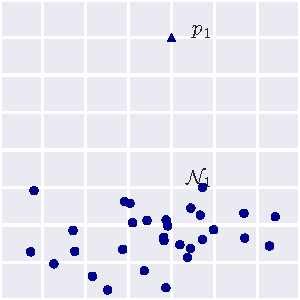
\includegraphics{figs/simple_dist.pdf}
  \caption{Simple Anomaly Distribution}
  \label{fig:simple_dist}
\end{figure}

Practically, this idealization never occurs. It is not as simple to distinguish $p_1$ and $p_2$ from $\mathcal{N}_1$ and $\mathcal{N}_2$ in the situations depicted in Figure \ref{fig:hard_dist}.

\begin{figure}[H]
  \centering
  \begin{subfigure}[H]{2in}
    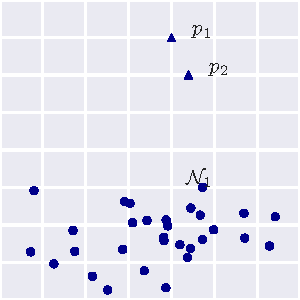
\includegraphics{figs/hard1_dist.pdf}
    \caption{}
    \label{fig:hard1_dist}
  \end{subfigure}
  \begin{subfigure}[H]{2in}
    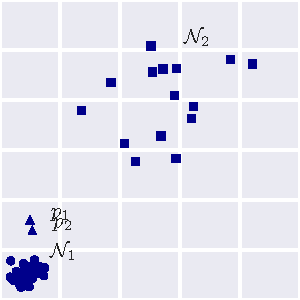
\includegraphics{figs/hard2_dist.pdf}
    \caption{}
    \label{fig:hard2_dist}
  \end{subfigure}
  \caption{Complex Anomaly Distribution}
  \label{fig:hard_dist}
\end{figure}

Having complex distributions is the purview of anomaly detection in general and not a problem particular to time series data. However, issues influenced by the temporal nature of the data will the focus of the next two subsections.

\subsection{Distance Measures}



%%% Local Variables:
%%% mode: latex
%%% TeX-master: "thesis"
%%% End: